\section{问题分析与建模思路}
第一问要求计算圆柱形药材在预热阶段 $1800\,\mathrm{s}$ 内的温度与干基含水率，并逐秒输出径向结果。药材长 $L=0.25\,\mathrm{m}$、半径 $R=0.02\,\mathrm{m}$，初始温度 $T_0=28\,\celsius$、含水率 $C_0=2.55\,\kgkg$。题给参数\cite{problem}为
\[
\rho=820\,\mathrm{kg/m^3},\quad c_p=2600\,\mathrm{J/(kg\cdot K)},\quad
k=0.36\,\mathrm{W/(m\cdot K)},
\]
\[
h=25\,\mathrm{W/(m^2\cdot K)},\quad k_m=8\times10^{-7}\,\mathrm{m/s},\quad
D(C)=7\times10^{-9}e^{-0.89/C}\,\mathrm{m^2/s}.
\]

\subsection{从物理尺度确定空间分辨的必要性}
令热扩散率 $\alpha=k/(\rho c_p)$、初始水分扩散率 $D_i=D(C_0)$。以半径 $R$ 为特征长度，定义热、质 Biot 数与 Fourier 数，得到下列尺度。
\begin{center}\small
\begin{tabular}{lll}
\toprule
指标 & 定义 & 数值\\\midrule
热、质扩散率之比 & $\alpha/D_i$ & $\DiffusivityRatio$\\
热 Biot 数 & $hR/k$ & $\BiHeat$\\
质 Biot 数 & $k_mR/D_i$ & $\BiMass$\\
热 Fourier 数（1800秒） & $\alpha t/R^2$ & $\FoHeat$\\
质 Fourier 数（1800秒） & $D_it/R^2$ & $\FoMass$\\
\bottomrule
\end{tabular}\end{center}
热扩散比初始水分扩散快约34倍，预示中心升温与外层失水具有不同的进程；两个 Biot 数均不很小，内部梯度与表面交换均应保留。初始系数对应的扩散长度 $\sqrt{\alpha t}$ 与 $\sqrt{D_it}$ 分别约为 $\HeatLength\,\mathrm{cm}$、$\MoistureLength\,\mathrm{cm}$，为网格在表面附近加密提供了尺度依据。它们仅表示扩散尺度，不是具有锐利分界的影响区域。

\subsection{有限圆柱主模型与中截面输出}
取圆柱中心为原点，$r,z$ 分别为径向、轴向坐标。利用轴对称性及中截面对称性，计算半域
\begin{equation}
\Omega=\{(r,z):0\le r\le R,\ 0\le z\le H\},\qquad H=L/2.
\label{eq:domain}
\end{equation}
轴对称体积元为 $\dd V=2\pi r\,\dd r\,\dd z$，$|\Omega|=\pi R^2H$。结果表中的“到药材中心距离”统一取\textbf{中截面 $z=0$ 上的径向距离 $r$}。二维模型保留端面交换；同物性的一维径向模型作为中截面数值参照，从而分别检验表格结果与端面影响。

\subsection{基本假设}
\begin{enumerate}
\item 药材为连续、均匀、各向同性介质，初始状态均匀，几何尺寸固定，采用题给有效热物性；干物质体积密度空间均匀且固定。
\item 烘房环境在空间上均匀、随时间变化，侧面和两端面均暴露，使用相同的换热、传质系数。
\item 取 $\Ceq=C_\infty$ 为等效平衡含水率的经验闭合；不加入参数不完整的吸附、蒸发潜热及辐射机制，其影响作为适用性限制讨论。
\end{enumerate}

\section{温度与水分迁移模型}

\subsection{时变环境边界}
在附件1中截取 $0$ 至 $1800\,\mathrm{s}$ 的31个采样点，不作平滑或外推。对任一环境变量 $B\in\{\Tin,C_\infty\}$，在相邻采样时刻 $t_j,t_{j+1}$ 之间取
\begin{equation}
 B(t)=B_j+\frac{t-t_j}{t_{j+1}-t_j}(B_{j+1}-B_j),\qquad t_j\le t\le t_{j+1}.
 \label{eq:ambient}
\end{equation}
由此保留环境温湿度的实际变化，并避免预先设定恒温段。两端时刻的环境温度分别为 $28\,\celsius$ 和 $41.513\,\celsius$，环境水分数据分别为 $0.01963\,\kgkg$ 和 $0.03307\,\kgkg$。

\subsection{控制方程}
根据能量守恒与傅里叶定律，轴对称温度场满足
\begin{equation}
 \rho c_p\frac{\partial T}{\partial t}
 =\frac{1}{r}\frac{\partial}{\partial r}\left(rk\frac{\partial T}{\partial r}\right)
  +\frac{\partial}{\partial z}\left(k\frac{\partial T}{\partial z}\right).
 \label{eq:heat}
\end{equation}
在固定干物质体积密度的假设下，将水分守恒式中的该密度约去，得到
\begin{equation}
 \frac{\partial C}{\partial t}
 =\frac{1}{r}\frac{\partial}{\partial r}\left(rD(C)\frac{\partial C}{\partial r}\right)
  +\frac{\partial}{\partial z}\left(D(C)\frac{\partial C}{\partial z}\right),\quad
 D(C)=7\times10^{-9}\exp\left(-\frac{0.89}{C}\right).
 \label{eq:moisture}
\end{equation}
式\eqref{eq:moisture}必须保留散度形式。由于 $D$ 随 $C$ 变化，展开后有
\begin{equation}
 \nabla\!\cdot[D(C)\nabla C]
 =D(C)\Delta C+D'(C)|\nabla C|^2,\qquad
 D'(C)=\frac{0.89}{C^2}D(C).
 \label{eq:nonlinear}
\end{equation}
直接使用 $D(C)\Delta C$ 会遗漏非线性梯度项。第一问中热物性均为常数，且 $D$ 仅依赖 $C$，因此温度方程与水分方程可以分别求解。

\subsection{初始条件及边界条件}
初始状态为
\begin{equation}
 T(r,z,0)=T_0,\qquad C(r,z,0)=C_0.
 \label{eq:initial}
\end{equation}
在中心轴和中截面分别施加对称条件
\begin{equation}
 \left.\frac{\partial T}{\partial r}\right|_{r=0}
 =\left.\frac{\partial C}{\partial r}\right|_{r=0}=0,\qquad
 \left.\frac{\partial T}{\partial z}\right|_{z=0}
 =\left.\frac{\partial C}{\partial z}\right|_{z=0}=0.
 \label{eq:symmetry}
\end{equation}
令 $\Gamma_e=\{r=R\}\cup\{z=H\}$ 为半域的暴露边界，$\bm n$ 为外法向，$T_s,C_s$ 为表面未知量，则
\begin{equation}
 \begin{aligned}
 -k\nabla T\cdot\bm n&=h(T_s-\Tin),\\
 -D(C_s)\nabla C\cdot\bm n&=k_m(C_s-\Ceq),\qquad \Ceq=C_\infty.
 \end{aligned}
 \label{eq:robin}
\end{equation}
该符号约定下，表面较环境冷时热流向内，表面含水率较高时水分向外迁移。表面状态由式\eqref{eq:robin}求解，而非直接赋成环境值。侧面与端面交界处分别计算两个方向的通量。初始均匀含水率与瞬时失水边界在 $t=0$ 不相容，需保留题设初值并在时间离散中解析启动层。


\clearpage
\section{守恒离散与初始边界层分辨}
\subsection{轴线与暴露表面的统一通量处理}
采用节点中心有限体积法，节点包含中心轴、对称中截面及真实外表面。内部控制面位于相邻节点中点，边界控制体截断于物理表面。对控制体 $P$，体积与两个方向的面面积为
\begin{equation}
V_P=\pi(r_+^2-r_-^2)(z_+-z_-),\quad
A_{r,\pm}=2\pi r_\pm(z_+-z_-),\quad A_{z,\pm}=\pi(r_+^2-r_-^2).
\label{eq:volume}
\end{equation}
其中 $r_\pm,z_\pm$ 为控制面坐标。中心轴处 $A_{r,-}=0$，离散时无需直接计算 $1/r$；端侧交界控制体分别计入侧面与端面的通量。

用 $u$ 统一表示温度或含水率，并定义
\[
(u,m,\kappa,\beta,u_e)=
\begin{cases}(T,\rho c_p,k,h,\Tin),&\text{热量方程},\\
(C,1,D(C),k_m,\Ceq),&\text{水分方程}.
\end{cases}
\]
记 $N(P)$ 为相邻节点集，$\mathcal E(P)$ 为暴露面集，$\ell_{PQ}$ 为节点间距，则
\begin{equation}
mV_P\dot u_P=\sum_{Q\in N(P)}\frac{A_{PQ}\kappa_{PQ}}{\ell_{PQ}}(u_Q-u_P)
 +\sum_{f\in\mathcal E(P)}\beta A_f(u_e-u_P).
\label{eq:fvm}
\end{equation}
水分面系数取调和平均 $D_{PQ}=2D(C_P)D(C_Q)/[D(C_P)+D(C_Q)]$。同一内部面的通量在相邻控制体中等量反向，全域求和后只剩外边界交换，保证离散收支一致。

\subsection{新时间层内更新非线性扩散率}
令 $M_C=\operatorname{diag}(V_P)$，将水分半离散式写为 $M_C\dot{\bm C}=L(\bm C)\bm C+\bm b(t)$；$L$ 包含内部扩散和 Robin 边界负对角项。采用非线性 Crank--Nicolson 格式，每步用 Picard 迭代求解：
\begin{equation}
\begin{aligned}
\left[M_C-\frac{\Delta t_n}{2}L(\bm C^{(m)})\right]\bm C^{(m+1)}
={}&M_C\bm C^n+\frac{\Delta t_n}{2}\bigl[L(\bm C^n)\bm C^n\\
&+\bm b(t_n)+\bm b(t_{n+1})\bigr].
\end{aligned}
\label{eq:picard}
\end{equation}
初猜为 $\bm C^{(0)}=\bm C^n$。旧层算子固定，新层扩散率随迭代更新；同时检查最大增量小于 $2\times10^{-10}$、非线性代数残差经 $M_C^{-1}$ 归一化后小于 $2\times10^{-9}\,\kgkg$。温度方程系数固定，使用相同时间格式直接求解线性系统。

\subsection{面向逐秒输出的空间加密与分级启动}
主网格取865个径向节点、25个半轴向节点。径向最后 $1\,\mathrm{mm}$ 加密，最大间距为 $0.03125\,\mathrm{mm}$，最小间距为 $3.90625\,\mu\mathrm m$；轴向向端面加密。求解网格包含全部要求的径向输出位置。

主步长为 $0.5\,\mathrm{s}$。先在 $[0,10^{-4}]\,\mathrm{s}$ 内执行两个隐式 Euler 半步，再按启动节点 $0.001$、$0.01$、$0.1$、$1$、$10$ 和 $60\,\mathrm{s}$ 逐级放宽步长，之后使用主步长。该安排解析初值与表面排湿不相容引起的薄边界层，并落在每个整数秒输出时刻。全过程不裁剪含水率，逐步检查正值性、温度范围与非线性收敛；主运行每步最多4次 Picard 迭代。下文用相同物理模型的对照计算评价加密与启动的收益。

\clearpage
\section{计算结果与预热过程解释}
\subsection{指定时刻的中截面结果}
由二维主模型提取 $T(r,0,t)$ 与 $C(r,0,t)$，按题目格式得到表\ref{tab:temperature}和表\ref{tab:moisture}。两表和完整 \texttt{result1.xlsx} 来自同一主解，含水率采用干基量，结果保留四位小数。
\begin{table}[H]
\centering\small
\caption{30分钟内中截面温度（单位：$\celsius$）}\label{tab:temperature}
\begin{tabular}{crrrrr}
\toprule
\multirow{2}{*}{时间 / s} & \multicolumn{5}{c}{到药材中心的距离 / cm}\\
\cmidrule(lr){2-6} & 0 & 0.5 & 1 & 1.5 & 2\\
\midrule
100 & 28.0001 & 28.0003 & 28.0040 & 28.0327 & 28.1801 \\
300 & 28.0408 & 28.0635 & 28.1514 & 28.3681 & 28.8489 \\
600 & 28.4533 & 28.5360 & 28.8039 & 29.3159 & 30.1652 \\
900 & 29.3243 & 29.4583 & 29.8755 & 30.6161 & 31.7304 \\
1200 & 30.5427 & 30.7098 & 31.2223 & 32.1126 & 33.4276 \\
1500 & 31.9957 & 32.1867 & 32.7660 & 33.7463 & 35.1203 \\
1800 & 33.5753 & 33.7720 & 34.3642 & 35.3621 & 36.7856 \\
\bottomrule
\end{tabular}
\end{table}

\begin{table}[H]
\centering\small
\caption{30分钟内中截面干基含水率（单位：$\kgkg$）}\label{tab:moisture}
\begin{tabular}{crrrrr}
\toprule
\multirow{2}{*}{时间 / s} & \multicolumn{5}{c}{到药材中心的距离 / cm}\\
\cmidrule(lr){2-6} & 0 & 0.5 & 1 & 1.5 & 2\\
\midrule
100 & 2.5500 & 2.5500 & 2.5500 & 2.5500 & 2.2471 \\
300 & 2.5500 & 2.5500 & 2.5500 & 2.5492 & 2.0508 \\
600 & 2.5500 & 2.5500 & 2.5500 & 2.5353 & 1.8770 \\
900 & 2.5500 & 2.5500 & 2.5497 & 2.5045 & 1.7547 \\
1200 & 2.5500 & 2.5500 & 2.5482 & 2.4646 & 1.6586 \\
1500 & 2.5500 & 2.5499 & 2.5445 & 2.4206 & 1.5787 \\
1800 & 2.5500 & 2.5497 & 2.5383 & 2.3755 & 1.5102 \\
\bottomrule
\end{tabular}
\end{table}

在 $1800\,\mathrm{s}$ 时，中截面中心与侧面温度分别为 $\FinalCenterT\,\celsius$、$\FinalSurfaceT\,\celsius$；含水率分别为 $\FinalCenterC\,\kgkg$、$\FinalSurfaceC\,\kgkg$。中心与侧面仍分别比烘房低约 $\CenterGap\,\celsius$、$\SurfaceGap\,\celsius$，说明热量已传至中心，但该时段尚未达到热平衡。

表中中心含水率显示为 $2.5500$，仅表示四位小数舍入后的结果，并非该位置严格没有变化。完整文件分别保存温度和水分浓度的 $1800\times21$ 个结果，覆盖每隔1秒、径向每隔0.1厘米的位置。

\clearpage
\subsection{径向剖面与特征位置时程}
图\ref{fig:profiles}显示外层先升温、先失水；图\ref{fig:history}进一步将特征位置与时变环境对照。水分在表层变化较快，中心变化很小；温度则在整个径向范围内逐渐抬升，与热、质 Fourier 数的尺度差异一致。
\begin{figure}[H]\centering
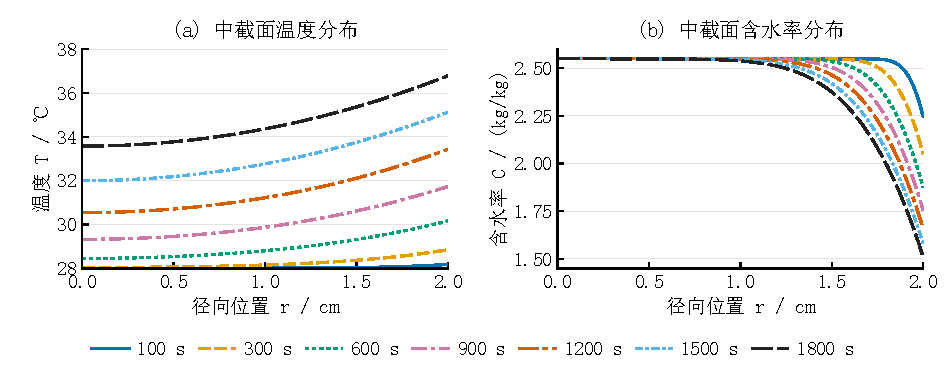
\includegraphics[width=\linewidth]{figures/q1_radial_profiles.pdf}
\caption{七个指定时刻的中截面剖面：外层温度较高、含水率较低。}
\label{fig:profiles}\end{figure}
\begin{figure}[H]\centering
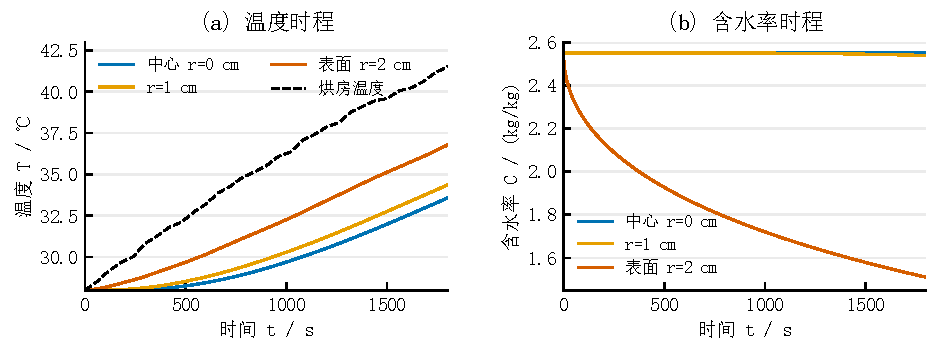
\includegraphics[width=\linewidth]{figures/q1_history.pdf}
\caption{中心、半径1厘米与表面的时间变化。温度图附烘房数据，体现内部响应的滞后。}
\label{fig:history}\end{figure}

为量化外层失水的影响范围，定义含水率相对初值下降 $\varepsilon$ 时的阈值半径与壳层厚度：
\begin{equation}
r_\varepsilon(t)=\inf\{r:C(r,0,t)\le(1-\varepsilon)C_0\},\qquad
\delta_\varepsilon(t)=R-r_\varepsilon(t).
\label{eq:front}
\end{equation}
集合为空时记为阈值尚未达到。根据未舍入的径向快照插值，1800秒时下降1\%和5\%对应的外层厚度分别约为 $\DepthOne\,\mathrm{cm}$、$\DepthFive\,\mathrm{cm}$。该量提供明确的分布描述，阈值由分析目的指定，不将其解释为真实锐利相界面。

\clearpage
\section{数值验证与关键处理的收益}
\subsection{中截面收敛与逐项对照}
以全部 $1800\times21$ 个中截面输出点的最大绝对差作为比较指标，表\ref{tab:verification}给出同网格一维对照及加密结果。时间加密将一维主步长由0.5秒减至0.25秒；空间加密在0.25秒下将径向节点由865增至1729。该比较检验实际环境驱动下的整个输出时段。
\begin{table}[H]
\centering\small
\caption{全部中截面输出点的最大绝对差}\label{tab:verification}
\begin{tabular}{lrr}
\toprule
比较内容 & 温度 / $\celsius$ & 含水率 / $(\kgkg)$\\
\midrule
二维中截面与同网格一维对照 & $3.74\times10^{-7}$ & $2.21\times10^{-12}$ \\
一维时间步长减半 & $5.35\times10^{-7}$ & $3.88\times10^{-7}$ \\
一维径向网格加密一倍 & $1.13\times10^{-6}$ & $8.38\times10^{-6}$ \\
二维中截面与更细一维参考 & $1.64\times10^{-6}$ & $8.41\times10^{-6}$ \\
\bottomrule
\end{tabular}
\end{table}


进一步使用同一1729节点、0.25秒一维解作为参考，仅改变网格分布或启动安排，得到表\ref{tab:ablation}。均匀网格取881节点以包含全部输出位置，比加密网格节点数约多1.8\%，属于相近计算规模的比较。
\begin{table}[H]
\centering\small
\caption{相近径向网格下的局部加密与启动层对照}\label{tab:ablation}
\begin{tabular}{lrrrr}
\toprule
径向配置 & 节点数 & 温度最大差 & 含水率最大差 & 含水率早期最大差\\
\midrule
局部加密 + 分级启动（主） & 865 & $1.638\times10^{-6}$ & $8.414\times10^{-6}$ & $7.843\times10^{-6}$ \\
均匀网格 + 分级启动 & 881 & $9.393\times10^{-7}$ & $2.063\times10^{-4}$ & $2.063\times10^{-4}$ \\
局部加密 + 普通启动 & 865 & $7.001\times10^{-6}$ & $1.020\times10^{-4}$ & $1.020\times10^{-4}$ \\
\bottomrule
\end{tabular}
\end{table}

在此比较中，局部加密方案的含水率最大差较均匀网格约缩小 $\GridGain$ 倍；分级启动较普通启动约缩小 $\StartupGain$ 倍。两种对照的最大含水率差均出现在第1秒的表面，说明收益主要针对题目要求的早期逐秒输出。温度差均较小，局部加密并未在本次对照中同时改善所有热场指标。

只检查论文指定时刻会弱化这一差别：普通启动在7个指定时刻、5个半径上的含水率最大差仅为 $\StandardTableDifference\,\kgkg$。因此，网格与启动方案应按完整输出要求评价。上述差值是数值参照差，不是严格解析误差上界，也不保证每个舍入末位都一致。

\subsection{轴向加密与独立核验}
\begin{table}[H]
\centering\small
\caption{轴向加密对中截面与全域指标的影响}\label{tab:axial}
\begin{tabular}{lrr}
\toprule
指标 & 温度 / $\celsius$ & 含水率 / $(\kgkg)$\\
\midrule
25个半轴向节点 & $2.620\times10^{-7}$ & $4.642\times10^{-12}$ \\
49个半轴向节点 & — & — \\
全场快照差（最大） & $7.600\times10^{-3}$ & $1.271\times10^{-2}$ \\
1800 s体积均值差 & $4.192\times10^{-4}$ & $9.724\times10^{-5}$ \\
\bottomrule
\end{tabular}
\end{table}

温度另以分段线性环境驱动的贝塞尔级数径向解核查，二维中截面温度与其最大差为 $\AnalyticError\,\celsius$。按与时间推进一致的积分权重累计边界通量，归一化热量、水分收支最大残差分别为 $\HeatResidual\,\celsius$、$\WaterResidual\,\kgkg$；水分检查使用含水率体积分，转换为水质量还需一致定义的干物质密度。

\section{方法特色与适用范围}
本方案的特色集中于\textbf{针对题目输出要求组织几何、通量和分辨率}。有限圆柱主模型保留端面，一维参照单独核验中截面；控制体通量统一处理轴线、表面与端侧交界；局部网格加密和分级启动共同解析初始排湿边界层，其收益由相近节点数与相同参考解下的对照量化。无量纲尺度和阈值影响深度进一步把数值场转化为可解释的预热过程。以上采用已有数值工具形成适合本题的建模方案，不额外引入待辨识的物理参数。

结论的适用范围受三项条件限制：其一，$\Ceq=C_\infty$ 是经验闭合，空气水分数据与药材干基含水率之间缺少吸附平衡及质量基准转换；其二，未计入蒸发潜热和尺寸变化，不能据本次结果断言这些影响可忽略；其三，现有验证主要针对中截面，端部全场尚未获得同级精度证据。题目没有提供内部温湿度实测数据，本文的验证支持数值计算的一致性，不替代物理预测精度的实验检验。

\begin{thebibliography}{9}\small
\bibitem{problem} 2026年高教社杯全国大学生数学建模竞赛题目：A题药材的烘干问题[Z]. 2026. 问题1、附录2及附件1.
\end{thebibliography}
